\section{Programmazione multicore e multithreading}
Definiamo un \textbf{thread} come l'unità di base di uso della CPU, composto da un relativo identificatore, un program counter, un insieme di registri
e una stack di attivazione. Condivide con altri thread appartenenti allo stesso processo le sezioni di codice, dati e altre risorse, come per esempio
i file aperti.\par
Finora abbiamo parlato di \textbf{heavyweight processes}, ovvero quelli composti da un solo thread, mentre in questa sezione discuteremo degli scopi e
dei vantaggi della programmazione di processi \textbf{multithreaded}.\newline

\noindent La maggior parte delle applicazioni odierne è multithreaded; si codificano infatti come un processo a sé stante che comprende più thread di
controllo. Per esempio, un web browser ha un filo per rappresentare a schermo le pagine e un altro per scaricare i dati dalla rete. La ragione
principale per la quale si è passati da un paradigma monolitico al multithread è che sempre più spesso era necessario per le applicazioni saper gestire
più compiti allo stesso tempo; un web server intensamente utilizzato vede molti client che vi accedono concorrentemente, per esempio.\par
Una prima soluzione a questo problema sarebbe di creare un nuovo processo per ogni richiesta, ma risulterebbe estremamente oneroso in termini di risorse
e tempo. È nettamente più conveniente creare un thread apposito per ogni nuova richiesta, poiché condividendo le sezioni non è necessario allocare nuova
memoria.\par
Anche la maggior parte dei kernel dei sistemi operativi moderni è multithreaded; all'avvio di un sistema Linux vengono infatti creati diversi thread per
le varie attività da svolgere, come la gestione dei dispositivi o della memoria. Determinati algoritmi possono inoltre trarre vantaggio da questo
paradigma riducendo drasticamente i tempi di risposta.\newline

\noindent Possiamo raggruppare i vantaggi del paradigma multithread in quattro categorie principali: in primo luogo, si riducono i \textbf{tempi di
risposta}, perché consentiamo al programma di continuare la sua esecuzione mentre gestisce altre operazioni su diversi thread.\par
Richiamando come i processi comunichino, ovvero tramite memoria condivisa o scambio di messaggi, ai thread è possibile \textbf{condividere risorse} e
memoria del processo a cui appartengono.\par
Come già menzionato, la creazione di nuovi processi risulta più costosa rispetto alla generazione di nuovi thread, perché per questi ultimi si richiede
l'impiego di meno memoria, tempo, ed è anche più semplice gestirne il cambio di contesto.\par
Infine, i processi multithreaded sono facilmente \textbf{scalabili}; nelle architetture multiprocessore i thread si possono eseguire in parallelo,
incrementando il parallelismo.
\begin{figure}[h]
	\centering
	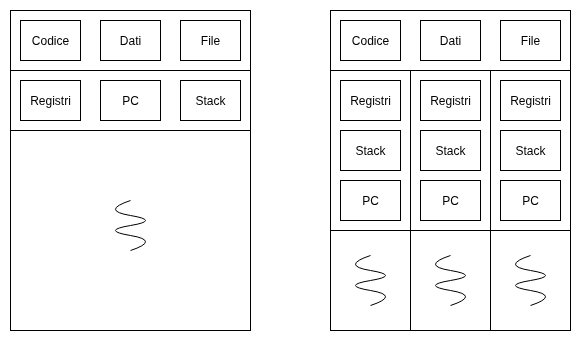
\includegraphics[width=0.9\linewidth]{Images/single_and_multithreaded_processes.png}
	\caption{Panoramica processi a singolo thread e multithreaded}
\end{figure}

\noindent In risposta alle necessità di maggiore potenza di calcolo, i calcolatori odierni presentano architetture multiprocessore, quindi che
dispongono di più core di elaborazione su un unico chip. La \textbf{programmazione multithread} definisce un meccanismo per l'utilizzo efficiente di
queste architetture, sfruttando al meglio la concorrenza.\par
Quando parliamo di \textbf{esecuzione concorrente} in questo contesto, intendiamo che i thread possono funzionare in parallelo perché il sistema può
assegnare thread diversi ad ogni core della CPU. Inoltre distinguiamo \textbf{sistema concorrente}, ovvero che supporta più task permettendo a ciascuno
di progredire nell'esecuzione, da \textbf{sistema parallelo}, dove è effettivamente possibile eseguire simultaneamente più compiti.
\begin{figure}[h]
	\centering
	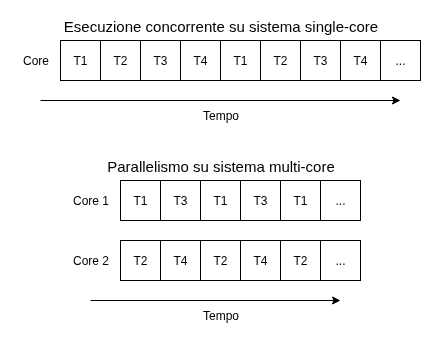
\includegraphics[width=0.7\linewidth]{Images/concurrence_and_parallelism.png}
	\caption{Panoramica concorrenza e parallelismo}
\end{figure}

\noindent Questo cambio di forma porta delle nuove sfide in ambito progettuale e di sviluppo applicazioni; chi crea e mantiene sistemi operativi dovrà
scrivere algoritmi di scheduling orientati all'utilizzo di più core e i programmatori di applicazioni dovranno renderle multithreaded. In particolare,
identifichiamo le seguenti sfide nella programmazione multicore: \begin{itemize}
	\item \textbf{Identificazione compiti}: Necessità di individuare aree separabili in task e quindi in thread.
	\item \textbf{Bilanciamento}: Le task devono eseguire compiti di mole e valore confrontabili. Se presentano un basso valore computazionale, potrebbe
	non valerne la pena di dedicarvi un intero core.
	\item \textbf{Suddivisione dati}: Definire i dati manipolati e a cui accedono le task. Vanno suddivisi per essere usati su core distinti.
	\item \textbf{Dipendenze dati}: In caso di dipendenze tra due o più task è necessario anche implementare un meccanismo di sincronizzazione per
	garantirne il corretto flusso di esecuzione.
	\item \textbf{Test e debugging}: Avendo più fili di esecuzione risulta più difficile fare testing e debugging.
\end{itemize}
\noindent Definiamo inoltre due tipi di parallelismo: quello dei \textbf{dati}, che riguarda la distribuzione di sottoinsiemi di dati su più core e
l'esecuzione di una stessa operazione su ognuno di essi, e il \textbf{parallelismo delle attività}, che distribuisce thread su più core, i quali possono
operare sugli stesso dati o diversi. Questi tipi di parallelismo non sono mutualmente esclusivi; infatti nei sistemi operativi è comune trovarne 
un'implementazione ibrida.
\begin{figure}[h]
	\centering
	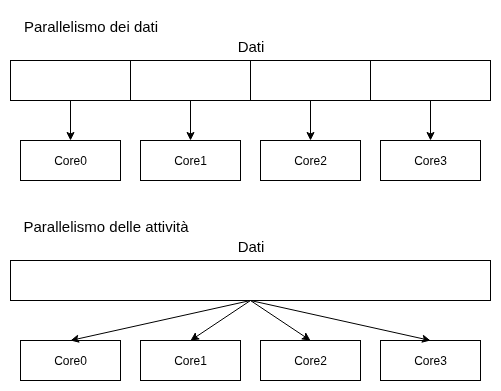
\includegraphics[width=0.9\linewidth]{Images/parallelism_types.png}
	\caption{Tipi di parallelismo}
\end{figure}

\noindent Distinguiamo i thread su due livelli: a \textbf{livello utente} sono gestiti sopra quello del kernel e senza il suo supporto, mentre a
\textbf{livello kernel} sono gestiti direttamente dal sistema operativo. È necessario che questi siano messi in relazione; esistono tre modelli
principali per implementarla: \begin{itemize}
	\item \textbf{Modello da molti a uno}: Fa corrispondere più thread utente ad un solo thread kernel. Si tratta di una gestione efficiente dei thread
	effettuata grazie ad un'apposita libreria nello spazio utente. Tuttavia, se il thread kernel invoca una system call bloccante, bloccherà l'intero
	processo. Inoltre, dato che un solo thread alla volta può accedere al kernel, è impossibile eseguire thread multipli in parallelo in sistemi
	multicore. Per queste ragioni è un modello raramente usato.
	\item \textbf{Modello da uno a uno}: Mette in corrispondenza ogni thread utente con un thread kernel, offrendo un maggiore grado di concorrenza e
	permettendo l'esecuzione in parallelo nei sistemi multiprocessore. Tuttavia, l'esistenza di un thread utente richiede quella del corrispondente
	thread kernel; essendo che questo meccanismo può sovraccaricare le prestazioni delle applicazioni, si sceglie di porre un limite al numero di
	thread supportabili, ma grazie alle architetture moderne si è potuto ridurre questa restrizione.
	\item \textbf{Modello da molti a molti}: Mette in corrispondenza più thread utente a un numero minore o uguale di thread kernel, dove il numero di
	thread kernel può essere calibrato in base all'applicazione o all'architettura del sistema. Per quanto riguarda la concorrenza, consente ai
	programmatori di creare liberamente un numero arbitrario di thread e i corrispondenti thread kernel si possono eseguire in parallelo nelle
	architetture multicore, superando gli svantaggi dei due precedenti modelli.\par
	Una variante di questo modello è il \textbf{modello a due livelli}, che mantiene la corrispondenza fra più thread utente e un numero minore o uguale
	di thread kernel, ma consente anche di vincolare un primo con un secondo, come per il modello uno a uno. Si tratta del modello più flessibile di
	tutti, ma è anche quello più difficile da implementare nella pratica.
\end{itemize}
\begin{figure}[h]
	\centering
	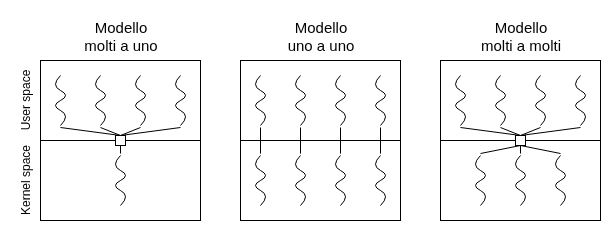
\includegraphics[width=0.9\linewidth]{Images/multithreading_models.png}
	\caption{Modelli di supporto multithreading}
\end{figure}

%

\section{Librerie dei thread}
Le librerie dei thread forniscono ai programmatori una API per la loro creazione e gestione. Ci sono due metodi principali per l'implementazione di
thread: collocare la \textbf{libreria a livello utente}, vedendo codice e strutture dati per la libreria risiedere nello spazio utente; invocare una
funzione implica una chiamata locale sul livello utente. Alternativamente è possibile collocare la \textbf{libreria a livello kernel}, facendo risiedere
le risorse nel relativo spazio e corrispondere l'invocazione di funzioni con le chiamate di sistema al kernel.\par
La libreria utilizzata in questo corso è \textbf{Pthreads}, di POSIX, la quale può essere realizzata in entrambe le modalità appena discusse. Con questa
API, tutti i dati dichiarati a livello globale sono condivisi tra tutti i thread generati dai programmi, mentre quelli a livello locale sono memorizzati
nello stack proprietario del filo, dando quindi ad ogni thread una propria copia dei dati locali.\newline

\noindent Esistono naturalmente più strategie per l'implementazione di thread: il \textbf{threading asincrono} vede il genitore creare un figlio e
continuare la sua esecuzione indipendentemente dal workflow del figlio, usato normalmente quando è richiesta una scarsa condivisione dei dati. Il
secondo metodo, invece, detto \textbf{threading sincrono}, blocca l'esecuzione del processo padre fino al termine dell'esecuzione dei
figli\footnote{Questa strategia è chiamata anche \textbf{fork-join}, perché il genitore attende che tutti i figli si ricongiungano col padre prima di
riprendere la sua esecuzione.}; generalmente è implementato quando vi è una significativa necessità di condivisione dati.\par
L'API fornito da Pthreads ci consente di implementare questi meccanismi in linguaggio C; sarà necessario includere la relativa libreria e usare le
funzioni apposite per inizializzare, creare e terminare thread di esecuzione. Prendiamo il seguente esempio: \begin{lstlisting}[language=C]
	# include <pthread.h>
	# include <stdio.h>
	# include <stdlib.h>
	
	int sum; // Variabile globale, condivisa dai thread in questo file
	void *runner(void *param); // Chiamata dai thread
	
	int main (int argc, char *argv[]) {
		pthread_t tid; // Identificatore del thread
		pthread_attr_t attr; // Insieme di attributi del thread
		
		// Inizializza thread con attributi predefiniti
		pthread_attr_init(&attr);
		// Crea il thread
		pthread_create(&tid, &attr, runner, argv[1]);
		// Attende terminazione thread figlio
		pthread_join(tid, NULL);
		
		printf("%d\n", sum);
	}
	
	// Thread eseguito nella seguente funzione runner
	void *runner (void *param) {
		int upper = atoi(param);
		sum = 0;
		
		for (int i = 1; i <= upper; i++) sum += i;
		
		pthread_exit(0);
	}
\end{lstlisting}

\noindent Il programma implementa un semplice workflow dove un processo padre genera un thread figlio, nel quale si ritorna la somma di tutti i numeri
fino al parametro passato in funzione.\par
Per creare un thread figlio, il padre deve in primo luogo assegnargli un identificativo e degli attributi, inizializzati tramite pthread\_attr\_init().
Dopodiché potrà generare il figlio con pthread\_create(), che prende in input questi due valori, la funzione dove è eseguito il thread e il parametro
ivi indicato. Per garantire un workflow sincrono, il padre usa pthread\_join() per fermare la sua esecuzione fin quando tutti i figli non hanno
terminato il loro lavoro.\par
È possibile naturalmente generare più thread; una strategia comune per la modalità sincrona è di implementare un ciclo for e un counter apposito che si
incrementa fino al termine di ogni figlio.

%

\section{Threading implicito}
Con la costante evoluzione della programmazione multicore si richiede anche la gestione di centinaia o migliaia di thread, comportando l'attuazione di
strategie per la progettazione delle applicazioni parallele o concorrenti. Una prima idea, detta \textbf{threading implicito}, vede il trasferimento
della creazione e gestione del threading ai compilatori e alle librerie. Richiede agli sviluppatori l'identificazione dei task da eseguire in parallelo,
i quali saranno codificati come funzioni.\par
Rimane tuttavia il problema del consumo delle risorse in base al numero di thread attivi. La soluzione è data dall'impiego dei \textbf{gruppi di thread},
quindi la creazione di un determinato numero di fili organizzati in gruppi all'attivazione del processo. La pool contiene i thread pronti ad eseguire
richieste; quando si attiva un task, viene prelevato un filo da questo gruppo e gli si assegna il compito. Esaudita la richiesta, potrà essere
reinserito nella pool. Questa strategia porta diversi vantaggi: \begin{itemize}
	\item Fornisce un servizio più rapido rimuovendo il ritardo dovuto alla creazione dinamica del thread.
	\item Limitando il numero di thread esistenti, consente l'esecuzione del programma anche su sistemi low-specs.
	\item Separare il task dalla meccanica della sua creazione dona modularità al sistema.
\end{itemize}
\noindent In particolare, il numero di thread massimo si può determinare in base ad alcuni fattori come il numero di core della CPU o la quantità di
memoria fisica disponibile.\par
La strategia di \textbf{fork-join} trattata nelle sezioni precedenti è un'altra modalità per l'implementazione di threading implicito; si possono
definire dei task paralleli la cui assegnazione ai thread è gestita dalla libreria di runtime. Questa è di fatto una realizzazione di un thread pool
sincronizzato in cui il processo padre attende il completamento di tutti i task prima di proseguire.

%

\section{Problemi di gestione multithread}
Come già discusso, la programmazione multithread e multicore include la gestione di diversi problemi. In primo luogo, se un thread invoca fork(), il
nuovo processo potrebbe contenere un duplicato di tutti i fili oppure del thread invocante, oppure, invocando exec(), il programma specificato come
parametro sostituirebbe l'intero processo chiamante insieme a tutti i suoi thread. Si necessita di un meccanismo per un controllo corretto.\par
Nei sistemi UNIX si usano i \textbf{segnali} per comunicare ai processi il verificarsi degli eventi; questi possono essere ricevuti in modalità
sincrona o asincrona, ma seguono entrambi lo stesso schema di generazione, invio a processo e gestione.\par
Per esempio, un programma potrebbe tentare un accesso illegale su alcune zone di memoria; in tal caso è inviato un \textbf{segnale sincrono} al processo
colpevole e si procederà con la sua terminazione. Quando un segnale è invece causato da un evento esterno al processo, questo lo riceve in modalità
\textbf{asincrona}. Generalmente i segnali si possono gestire in due modi: mediante un gestore \textbf{predefinito} del kernel oppure con uno definito
dall'utente. In particolare, la gestione può ignorare il segnale oppure richiedere la terminazione del processo, ma nei processi multithread è
necessario capire a quale thread bisogna inviarlo. Generalmente, esistono le seguenti istanze: \begin{itemize}
	\item Segnale inviato al thread al quale si riferisce.
	\item Segnale inviato ad ogni thread del processo.
	\item Segnale inviato a specifici thread del processo.
	\item Definizione di un thread specifico per ricevere i segnali.
\end{itemize}
\noindent Inoltre, il modo per recapitare il segnale dipende dal suo tipo; quelli sincroni vanno inviati al thread che ha generato l'evento, mentre per
gli asincroni può dipendere dal contesto. Per esempio, il comando bash per terminare i programmi Ctrl+C produce un segnale inviato ad ogni thread del
processo in esecuzione. La funzione standard per inviare un segnale nei sistemi UNIX è: \begin{center}
	kill(pid\_t pid, int signal)
\end{center}
\noindent La quale prende come parametri l'identificatore del processo (pid) al quale deve essere recapitato il particolare segnale (signal). La
funzione equivalente per Pthreads è invece: \begin{center}
	pthread\_kill(pthread\_t tid, int signal)
\end{center}
\noindent Che richiede gli stessi parametri della precedente. Essendo che i segnali devono essere gestiti una sola volta, questi sono generalmente
inviati al primo thread che non li blocca.\par
Consideriamo ora la \textbf{cancellazione dei thread}, l'operazione che permette la terminazione di un filo prima del completamento del suo compito.
Il thread da cancellare si dice \textbf{bersaglio} e la sua terminazione può avvenire in due modalità: \textbf{asincrona}, dove un thread fa
immediatamente terminare il target, e \textbf{differita}, che vede il bersaglio controllare periodicamente la presenza del segnale di un altro thread,
il quale comunica se deve essere terminato o meno. In particolare, possono presentarsi problemi con la cancellazione quando ci sono risorse assegnate
a un thread cancellato oppure se si termina un thread mentre sta aggiornando dati condivisi con altri fili. Quest'ultimo caso, se trattato con 
cancellazione asincrona, risulta particolarmente problematico perché il sistema operativo potrebbe non recuperare tutte le risorse ad esso assegnate.\par
Nell'API di Pthreads, la cancellazione si avvia tramite la funzione \textbf{pthread\_cancel()}, dove viene passato come parametro il thread id del filo
da terminare. Segue esempio: \begin{lstlisting}[language=C]
	pthread_t tid;
	
	// Crea il thread
	pthread_create(&tid, 0, worker, NULL);

	// Blocco di codice intermedio

	// Cancella il thread
	pthread_cancel(tid);

	// Attende la terminazione del thread
	pthread_join(tid, NULL)
\end{lstlisting}

\noindent Notare che la chiamata a pthread\_cancel() è solamente la richiesta di cancellazione, perché l'effettiva terminazione dipende in base
alle impostazioni per la gestione di terminazioni del thread di destinazione. In particolare, si può impostare uno stato di cancellazione e il suo tipo
usando una API, scegliendo tra le seguenti opzioni: \begin{table}[h]
	\centering
	\begin{tabular}{|c|c|c|}
		\hline
		\textbf{Modalità} & \textbf{Stato} & \textbf{Tipo}\\
		\hline
		Off & Disabilitato & -\\
		\hline
		Differita & Abilitato & Differito\\
		\hline
		Asincrona & Abilitato & Asincrono\\
		\hline
	\end{tabular}
\end{table}

\noindent Il tipo di cancellazione predefinito è il differito, secondo il quale la cancellazione avviene esclusivamente quando il thread raggiunge un
\textbf{punto di cancellazione}. La stragrande maggioranza delle chiamate di sistema bloccanti è vista come punto di cancellazione; una tecnica per
crearne uno su Pthreads è tramite la funzione \textbf{pthread\_testcancel()}. Effettuata la richiesta di cancellazione, è chiamata una funzione detta
\textbf{gestore della pulizia}, la quale rilascia ogni risorsa legata al thread per poi eliminarlo.\newline

\noindent Un altro dei vantaggi discussi della programmazione multithread è dato dalla condivisione dei dati tra i thread di uno stesso processo, ma
può capitare che sia richiesta una copia privata di certi dati, detti \textbf{dati specifici del thread} (TLS). Questi sono definiti come statici
all'interno del codice e sono quindi unici e visibili all'interno dell'intero file ove sono scritti. Pthreads include il tipo \textbf{pthread\_key\_t}
che fornisce una chiave specifica per ogni filo, la quale può essere utilizzata per accedere ai dati TLS.\par
Un'ultima questione da affrontare riguarda poi la comunicazione tra la libreria del kernel e quella per i thread, necessaria nel modello da molti a
molti e a due livelli. Questa struttura rende il numero di thread modificabile dinamicamente con lo scopo di ottenere prestazioni migliori e vede il
collocamento di una struttura dati intermedia tra i thread kernel e utente. Questa, detta \textbf{processo leggero} (LWP) svolge una funzione di
processore virtuale e ne esiste uno per ogni thread kernel. L'applicazione potrà utilizzare gli LWP per richiedere lo scheduling di un thread a livello
utente. Tuttavia, essendo collegati, se un thread kernel si blocca, così faranno anche l'LWP e il thread utente; per questa ragione, con lo scopo di
garantire un'esecuzione efficiente, è consigliato utilizzare un LWP per ogni chiamata di sistema concorrente bloccante.\par
In questo contesto, uno dei modelli di comunicazione tra libreria utente e kernel è detto \textbf{attivazione dello scheduler}; il quale attua la
seguente procedura: \begin{enumerate}
	\item Il kernel fornisce alle applicazioni gli LWP sui quali scheduleranno i thread utente. Segnalerà inoltre la presenza di eventi tramite la
	procedura di \textbf{upcall}\footnote{Un'istanza per innescarne una è per esempio quando un processo è sul punto di bloccarsi}.
	\item Le upcall sono gestite dalla libreria dei thread mediante un gestore eseguito su LWP. Si identifica il thread indicato nella chiamata.
	\item Il kernel assegna all'applicazione un nuovo LWP, la quale eseguirà un gestore upcall su di esso.
	\item Il gestore salva lo stato del thread bloccante e rilascia l'LWP sul quale stava venendo eseguito. Pianifica inoltre l'esecuzione di un altro
	thread sul nuovo LWP.
	\item Al verificarsi dell'evento atteso dal thread bloccante, precedentemente segnalato dal kernel, questo effettua una nuova upcall\footnote{
	Naturalmente, anche questa chiamata necessita di un LWP, seguendo il procedimento appena descritto.} alla libreria per comunicare che il thread
	bloccato è nuovamente disponibile per l'esecuzione.
	\item L'applicazione contrassegna il thread in questione come pronto ed esegue lo scheduling di uno dei fili appartenenti a questo gruppo su uno
	dei processori virtuali disponibili.
\end{enumerate}

\noindent Discutiamo adesso del funzionamento dei thread in ambiente Linux. Questo sistema operativo non distingue tra processi e thread e impiega per
entrambi il termine \textbf{task}. La chiamata fork() duplica un processo e clone() crea un nuovo thread; quest'ultima in particolare riceve come
parametro alcuni flag per stabilire le risorse del padre da condividere col figlio; questi sono: \begin{itemize}
	\item \textbf{CLONE\_FS}: Condivisione informazioni sul file system.
	\item \textbf{CLONE\_VM}: Condivisione dello stesso spazio di memoria.
	\item \textbf{CLONE\_SIGHAND}: Condivisione dei gestori dei segnali.
	\item \textbf{CLONE\_FILES}: Condivisione dei file aperti.
\end{itemize}

\noindent Questa condivisione a intensità variabile è possibile grazie al modo in cui i task sono strutturati nel kernel. Esiste infatti un'unica
struttura dati che si serve di puntatori ad altri tipi struct contenenti i dati effettivi. In questi termini, fork() crea un nuovo task insieme con una
copia di tutte le strutture dati del genitore, mentre clone() fa puntare il nuovo task alle strutture dati del genitore in base ai flag passati nella
funzione. Questa funzione può essere utilizzata anche per l'implementazione di \textbf{container}, una tecnica di virtualizzazione fornita dal sistema
operativo per la creazione di diversi sistemi Linux.